%% ==============
\chapter{Fundamentals}
\label{ch:Fundamentals}
%% ==============
This chapter introduces important concepts and research fundamentals that are premised throughout this work. Most of these concepts are fundamental in photorealistic rendering and thus only covered briefly with references to popular basic literature for further understanding of this topic. Chapter~\ref{ch:Prev} will continue to cover related work that also focuses on solving lightning with many lights, but not necessarily acts as a foundation for the techniques introduced in chapter~\ref{ch:PNEE}.


\section{Rendering equation}

In modern photorealistic rendering the rendering equation (\ref{eq:req}) plays a central role. It describes how much radiance $L$ is emitted and reflected from a point $x$ into direction $\omega$. This serves as a physically correct representation of light transport for most observable phenomena.

\begin{align}
\label{eq:req}
L(x, \omega) =  L_e(x, \omega) + \int_{\Omega}f_r(\omega_i, x, \omega) L_i(x, w_i)\cos\theta_i d\omega_i 
\end{align}

$L_e(x, \omega)$ describes the light emission at $x$ into direction $\omega$. The integral is adding up reflected light from (infinitely) many directions $\omega_i$ and multiplies it with the solid angle $\cos \theta_i$. $f_r(\omega_i, x, \omega)$ is called the Bidirectional Scattering Distribution Function (BSDF) and provides a factor of how much incoming light from $\omega_i$ is reflected to direction $\omega$ at point $x$. Usually the BSDF is split up into a BRDF (Bidirectional Reflectance Distribution Function) and BSSDF (Bidirectional Subsurface scattering Distribution Function) which describe the positive hemisphere and negative hemisphere (within the material) respectively. Lastly $L_i(x, \omega_i)$ describes the incoming radiance from direction $\omega_i$. To calculate $L_i(x, \omega_i)$ a raycast is needed into direction $-\omega$. Assuming the first intersection of this ray is named $y$ $L_i(x, \omega_i)$ can be rewritten as $L(y, -\omega_i)$. Then again, $L(y, -\omega_i)$ can be calculated with the rendering equation, recursively. It is apparent that this spawns an infinite number of possible light paths and thus infinite dimensions to calculate correct light transport. To solve this only a limited number of samples can be taken to estimate the integral, this technique is discussed in section~\ref{sec:montecarlo}.

\subsection{Radiometry}


So far, we spared the conversation about the measurement units. Also a few assumptions should be mentioned concerning the rendering equation. We assume that light ensues to the rules of geometric optics, while in fact light has a wave-particle-dualism nature. Additionally, most computer graphic models ignore rarely visible phenomena like Phosphorescenc, Lumineszenz, fluorescence and polarization. With this assumptions we define that both $L$ and and $L_e$ from the rendering equation are given as Radiance in $[W / (m^2sr)]$. The measurement units are assambled as follows.
\begin{align}
L = \frac{dE}{\cos \theta d\omega} = \frac{d^2\Phi}{dA\cos \theta d\omega} \qquad [W / (m^2 sr) ]
\end{align}


With $\cos \theta d\omega$ being the projected solid angle $\omega^\tau$ and $E$ being the incident light called Irrandiance, which describes the radiant flux per area.
\begin{align}
E = \frac{ d\Phi }{ dA } \qquad [W m^{-2} ]
\end{align}
Then the radiant flux $\Phi$ being the radiant energy per time given as

\begin{align}
 \Phi = \frac{dQ}{dt} \qquad [W]   
\end{align}

measured in Watt $[W = Js^{-1} ]$. And the radiant Energy $Q$ measured in Joule $[J]$.

\subsection{light sources}


The radiant flux of a point light can now be set as $\Phi_g$ in $[W]$. Assuming an isotropic emission the Intensity of a point light is given as
\begin{align}
 I = \frac{\Phi_g}{4\pi sr} \qquad [ W sr^{-1} ] .
\end{align}

The Irradiance (incident $L$) on a sphere with radius $r$ around the point light is then given as
\begin{align}
E_r =  \frac{\Phi_g}{4\pi r^2} \qquad [ W m^{-2} ] .
\end{align}

For an area $dA$ the solid angle is 

\begin{align}
d\omega = \frac{\cos \theta dA}{r^2}  
\end{align}


and thus the Irradiance is

\begin{align}
E(x) = \frac{ I(\omega) d\omega }{ dA } = \frac{ \Phi_g \cos \theta }{ 4 \pi r^2}.
\end{align}

…

\section{Sampling}


The rendering equation is not directly solvable because of infinite directions $\omega$ in the integral and infinite paths at every intersection; To be able to calculate a good estimation thereof we have to take a reasonable number of samples and calculate their average.

\subsection{Monte Carlo Integration}
\label{sec:montecarlo}











%% ==============
\section{Rendering equation}
\subsection{Radiometry}
\subsection{Raytracer}
\subsection{Light Path Expressions}
\subsection{Measurement Contribution Function}


%% ==============
\section{Sampling}

\subsection{Probablity Density Function}

\subsection{Cumulative Distribution Function}

\subsection{Inverse Transform Sampling}

\subsection{Monte Carlo Integration}
\label{sec:MC}

\subsection{Importance Sampling}
\label{sec:IS}


\begin{figure}
    \centering
    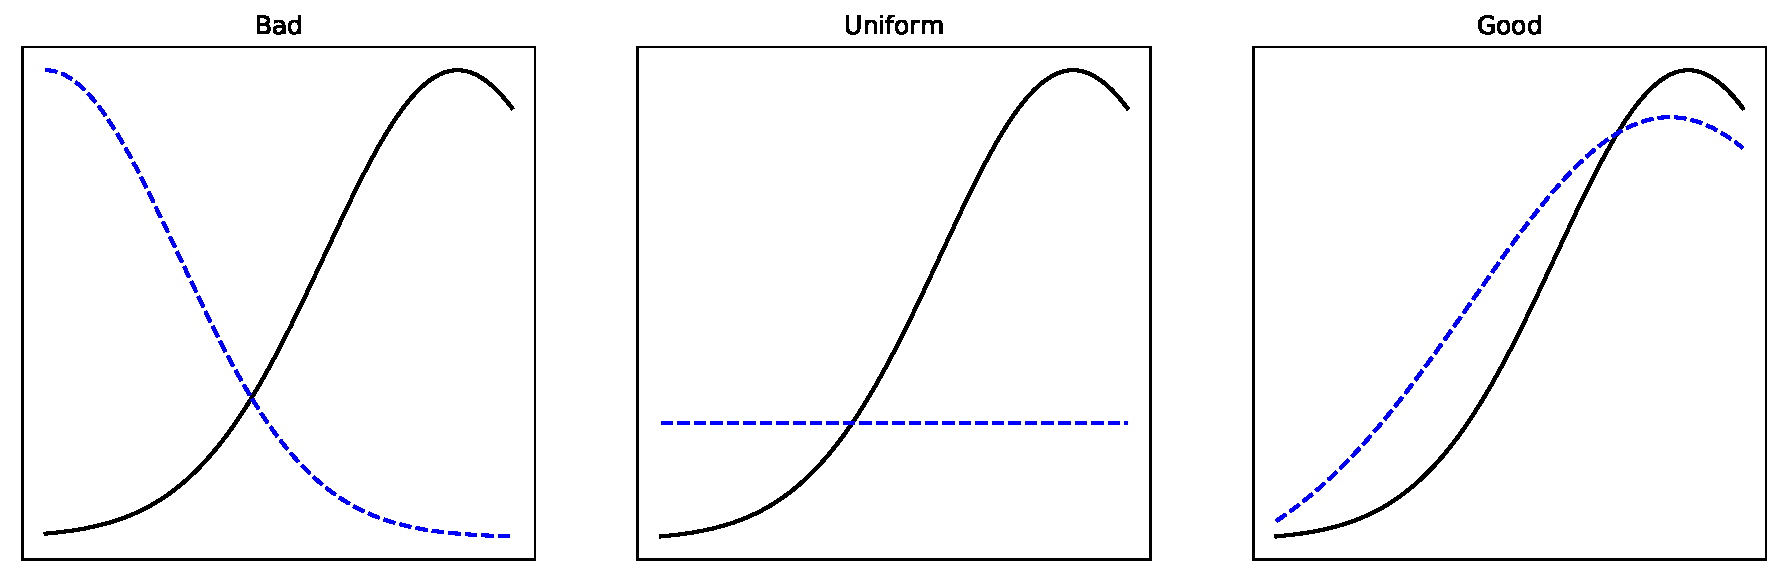
\includegraphics[width=0.8\textwidth]{figures/plots/importancesampling.pdf}
    \caption{.}
    \label{fig:importancesample}
\end{figure}

\subsection{Multiple Importance Sampling}

%% ==============
\section{Bidirectional scattering distribution function}
% mainly only for introduction of specular vs diffuse reflections


%% ==============
\section{Light sources}


%% ==============
\section{Path Tracing}
\subsection{Next Event Estimation}
\label{sec:NEE}


%% ==============
\section{Photon Mapping}
\label{sec:PM}

\subsection{Progressive Photon Mapping}

\subsection{Stochastic Progressive Photon Mapping}



%% ==============
\section{Instant Radiosity}

%% ==============
\section{Datastructures}

% Teapot in a stadium ...

\subsection{Bounding Volume Hierarchy}
\subsection{Grid}
\subsection{Octree}
\subsection{k-d Tree}
\subsection{Surface Area Heuristic}

\section{Interpolation}
\subsection{Scattered data}
\subsection{Structured data}

\label{ch:fu:trilinear}

\begin{figure}
    \centering
    
\includegraphics[width=0.5\textwidth]{figures/img-placeholder.png}
    \caption{The weights are the volume of the opposing rectangle.}
    \label{fig:bilinear}
\end{figure}
\subsection{Global methods}


%% ==============
\section{Machine Learning}

\subsection{Fuzzy k-means}
\subsection{Agglomerative Hierarchical Clustering}
\subsection{Expectation Maximaization}
\subsection{Transductive Support Vector Machine}